% This is samplepaper.tex, a sample chapter demonstrating the
% LLNCS macro package for Springer Computer Science proceedings;
% Version 2.20 of 2017/10/04
%
\documentclass[runningheads]{llncs}
%
\usepackage{graphicx}
\usepackage{hyperref}

\begin{document}
%
\title{Music Streaming and Song Recommendations Using ML Algorithms}
%
\author{Anthony M. Schomer}
%
\authorrunning{A. Schomer}
%
\institute{Northwest Missouri State University, Maryville MO 64468, USA \\
\email{tony.schomer@gmail.com}}
%
\maketitle              % typeset the header of the contribution
%
\begin{abstract}
This capstone project investigates the algorithms used by music streaming services to recommend similar songs to enhance user experiences. The focus is on how platforms like Spotify and Apple Music use listeners' preferences including likes, dislikes, and other relevant information to create personalized playlists tailored to individual tastes. This project uses open datasets such as Spotify Million Playlist Dataset, Spotify Web API, and Musicbrain.org's extensive library of databases. Using smart computer programs to create a test system that suggests songs based on user behavior and preferences. It looks at how current song recommendation systems work using machine learning methods such as collaborative filtering and content-based analysis to build test recommendation systems. This project also addresses challenges within the current algorithms to help avoid common issues. One significant issue to avoid is users hearing the same song over and over again. These findings will help improve music discovery online and suggest ways to innovate and enhance recommendations for listeners and introduce them to new artists.

\keywords{music \and streaming \and recommendations \and data \and user experience}
\end{abstract}

\section{Introduction}
[Your existing introduction content here]

\section{Data Processing and Methodology}

\subsection{Data Ingestion}
Our project utilized the Spotify Million Playlist Dataset, which contains 1 million playlists created by Spotify users. We accessed this data through the Spotify Web API, which provided a JSON format of playlist information including track details, audio features, and user interactions.

\subsection{Data Cleaning}
The raw data required several cleaning steps:
\begin{itemize}
    \item Removing duplicate tracks within playlists
    \item Handling missing values in audio features
    \item Standardizing genre labels
    \item Filtering out playlists with fewer than 10 tracks
\end{itemize}

We used Python's Pandas library for data manipulation and cleaning tasks.

\subsection{Analysis Process}
Our analysis involved several key steps:
\begin{enumerate}
    \item Exploratory Data Analysis (EDA) of audio features and playlist characteristics
    \item Feature engineering to create relevant input variables for our models
    \item Implementation of content-based and collaborative filtering algorithms
    \item Evaluation of model performance using metrics such as precision, recall, and mean average precision
\end{enumerate}

\section{Predictive Analysis and Model Building}

Our music recommendation system employs a hybrid approach combining content-based and collaborative filtering techniques. This section details the process of building and evaluating our predictive models.

\subsection{Feature Engineering}

We extracted audio features from the Spotify API, including tempo, energy, danceability, and acousticness. These features were combined with one-hot encoded genre information to create a comprehensive feature vector for each track.

\subsection{Exploratory Data Analysis}

Our analysis of audio features reveals interesting patterns in the dataset.

\subsection{Distribution of Audio Features}

Figure \ref{fig:audio_features} shows the distribution of key audio features such as danceability, energy, valence, and tempo.

\begin{figure}[h]
    \centering
    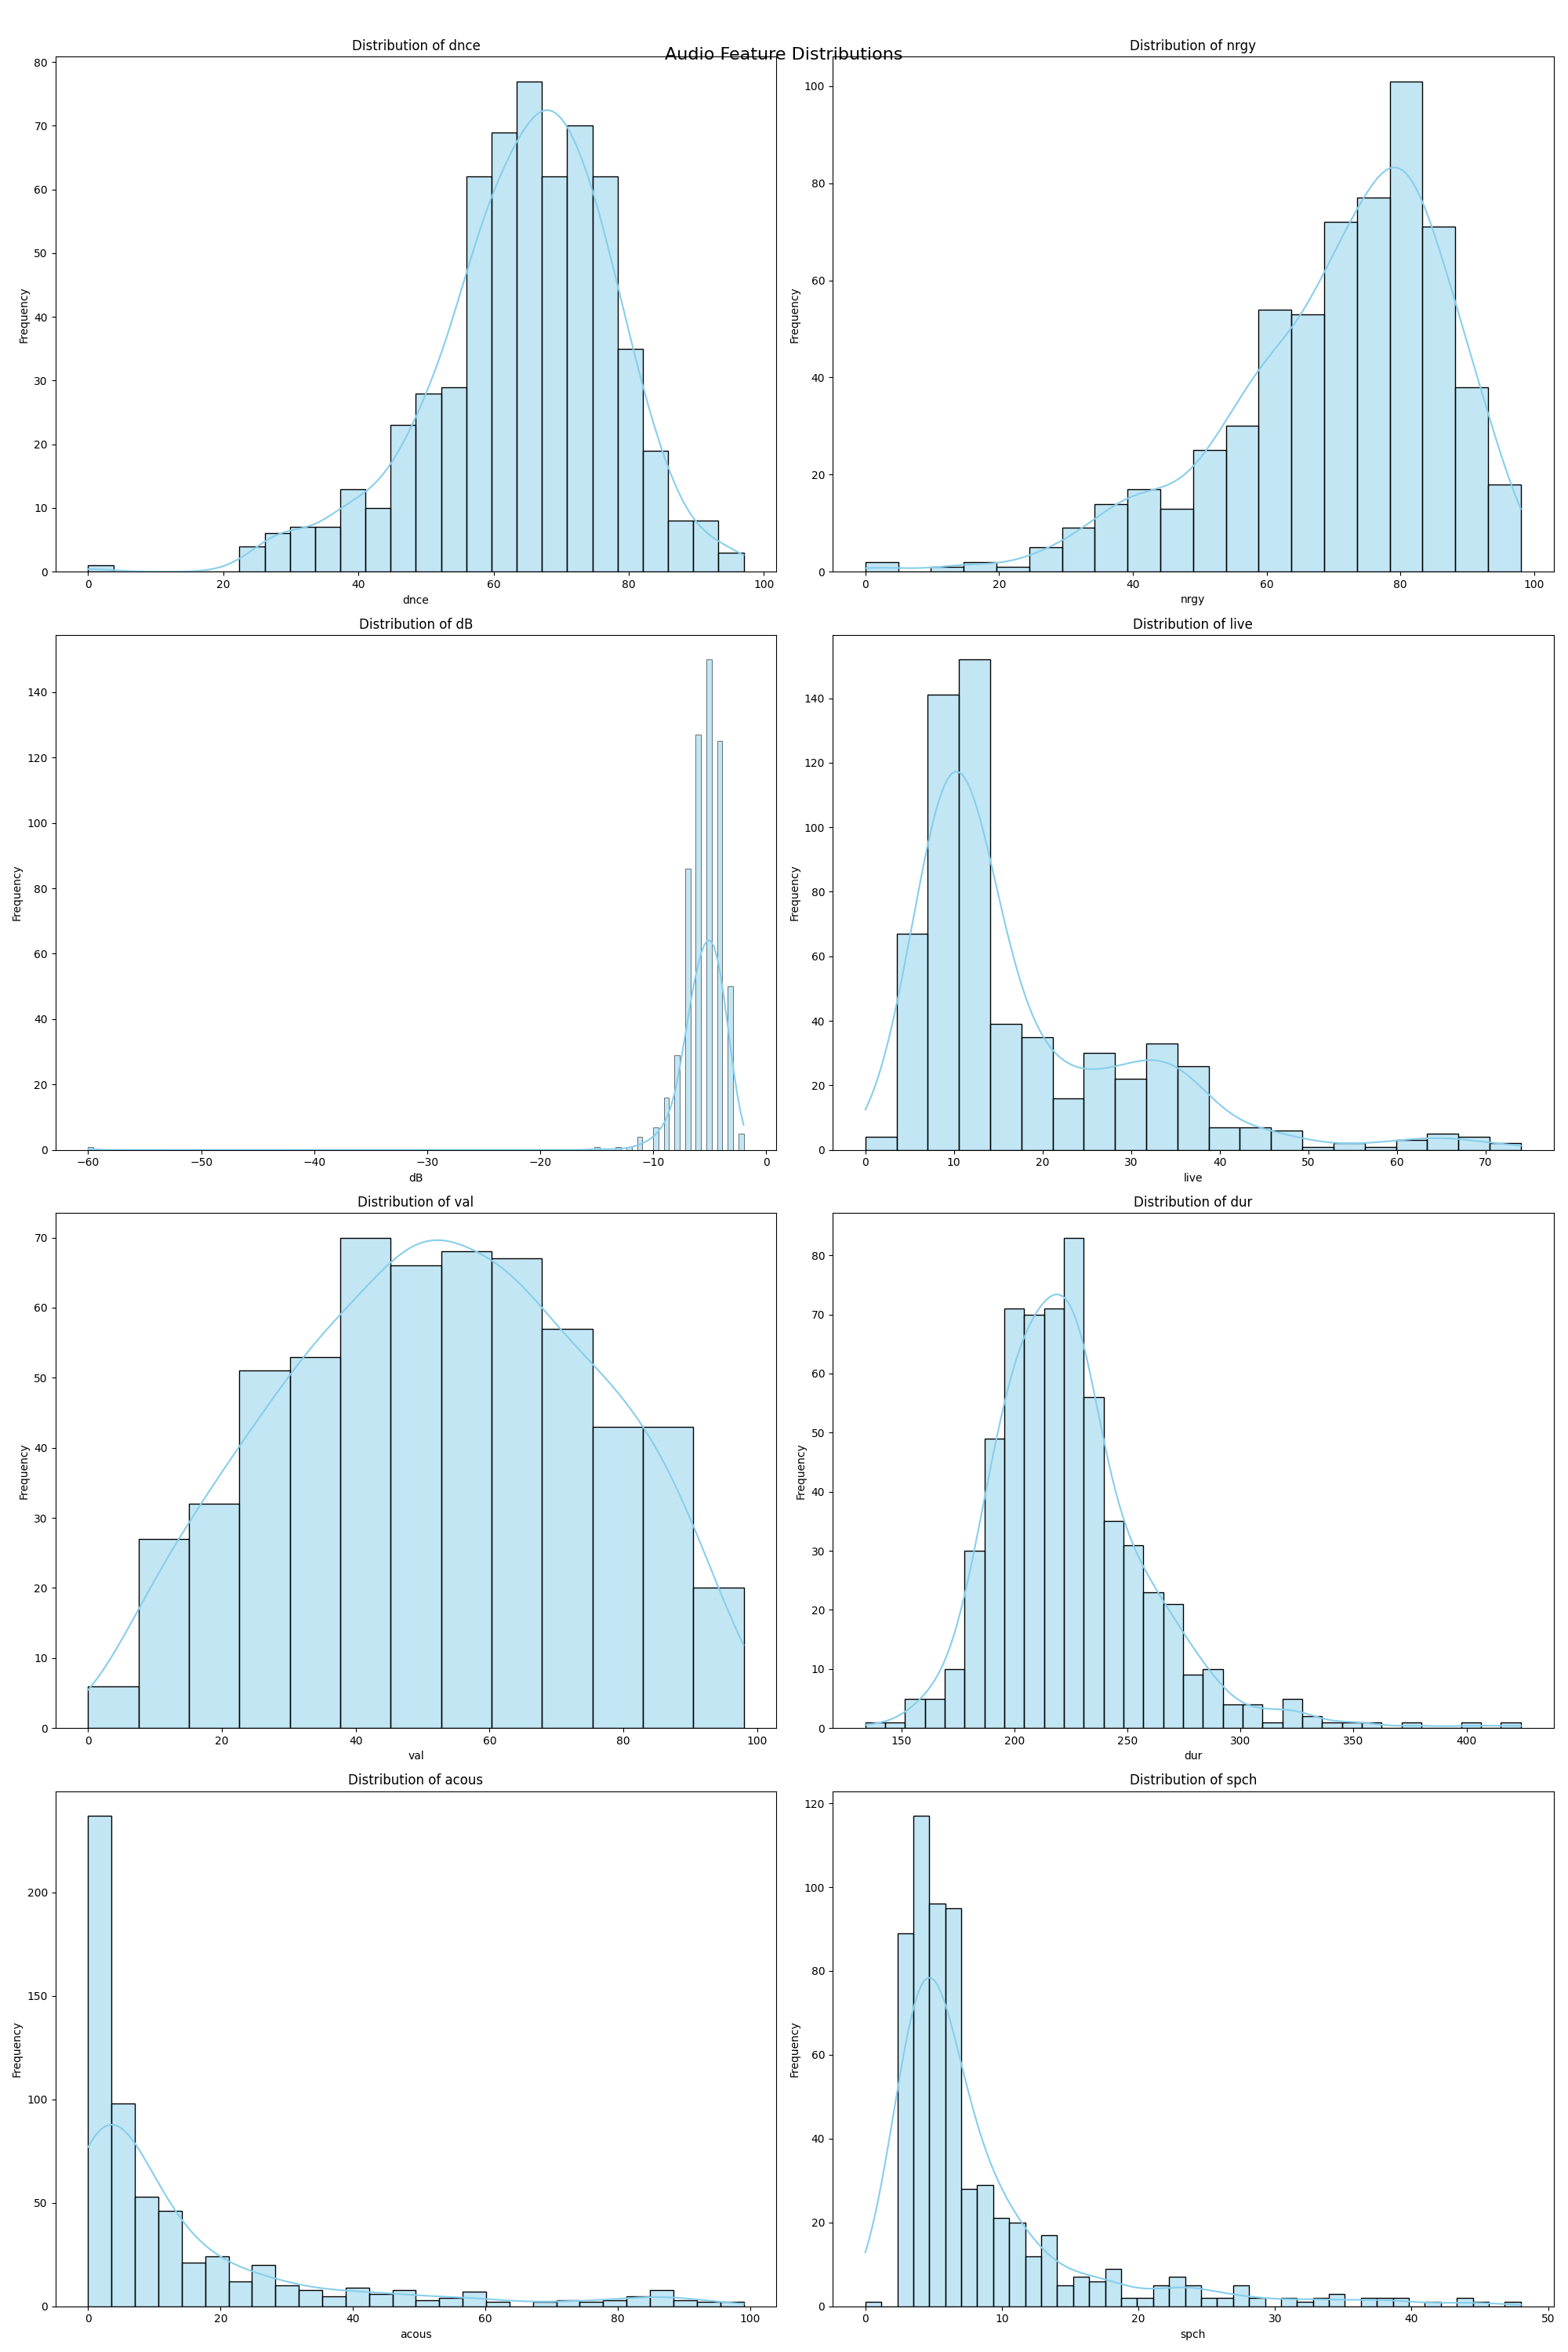
\includegraphics[width=0.8\textwidth]{audio_feature_distribution.png}
    \caption{Distribution of key audio features: danceability, energy, valence, and tempo. The histograms show that energy and danceability are relatively normally distributed, while valence has a slight positive skew.}
    \label{fig:audio_features}
\end{figure}

As shown in Figure \ref{fig:audio_features}, danceability and energy exhibit fairly normal distributions, suggesting a balanced range of songs in terms of these attributes. The valence distribution shows a slight positive skew, indicating a tendency towards more positive or upbeat songs in the dataset.

\subsection{Correlation Analysis}

Figure \ref{fig:correlation} presents the correlation between different audio features.

\begin{figure}[h]
    \centering
    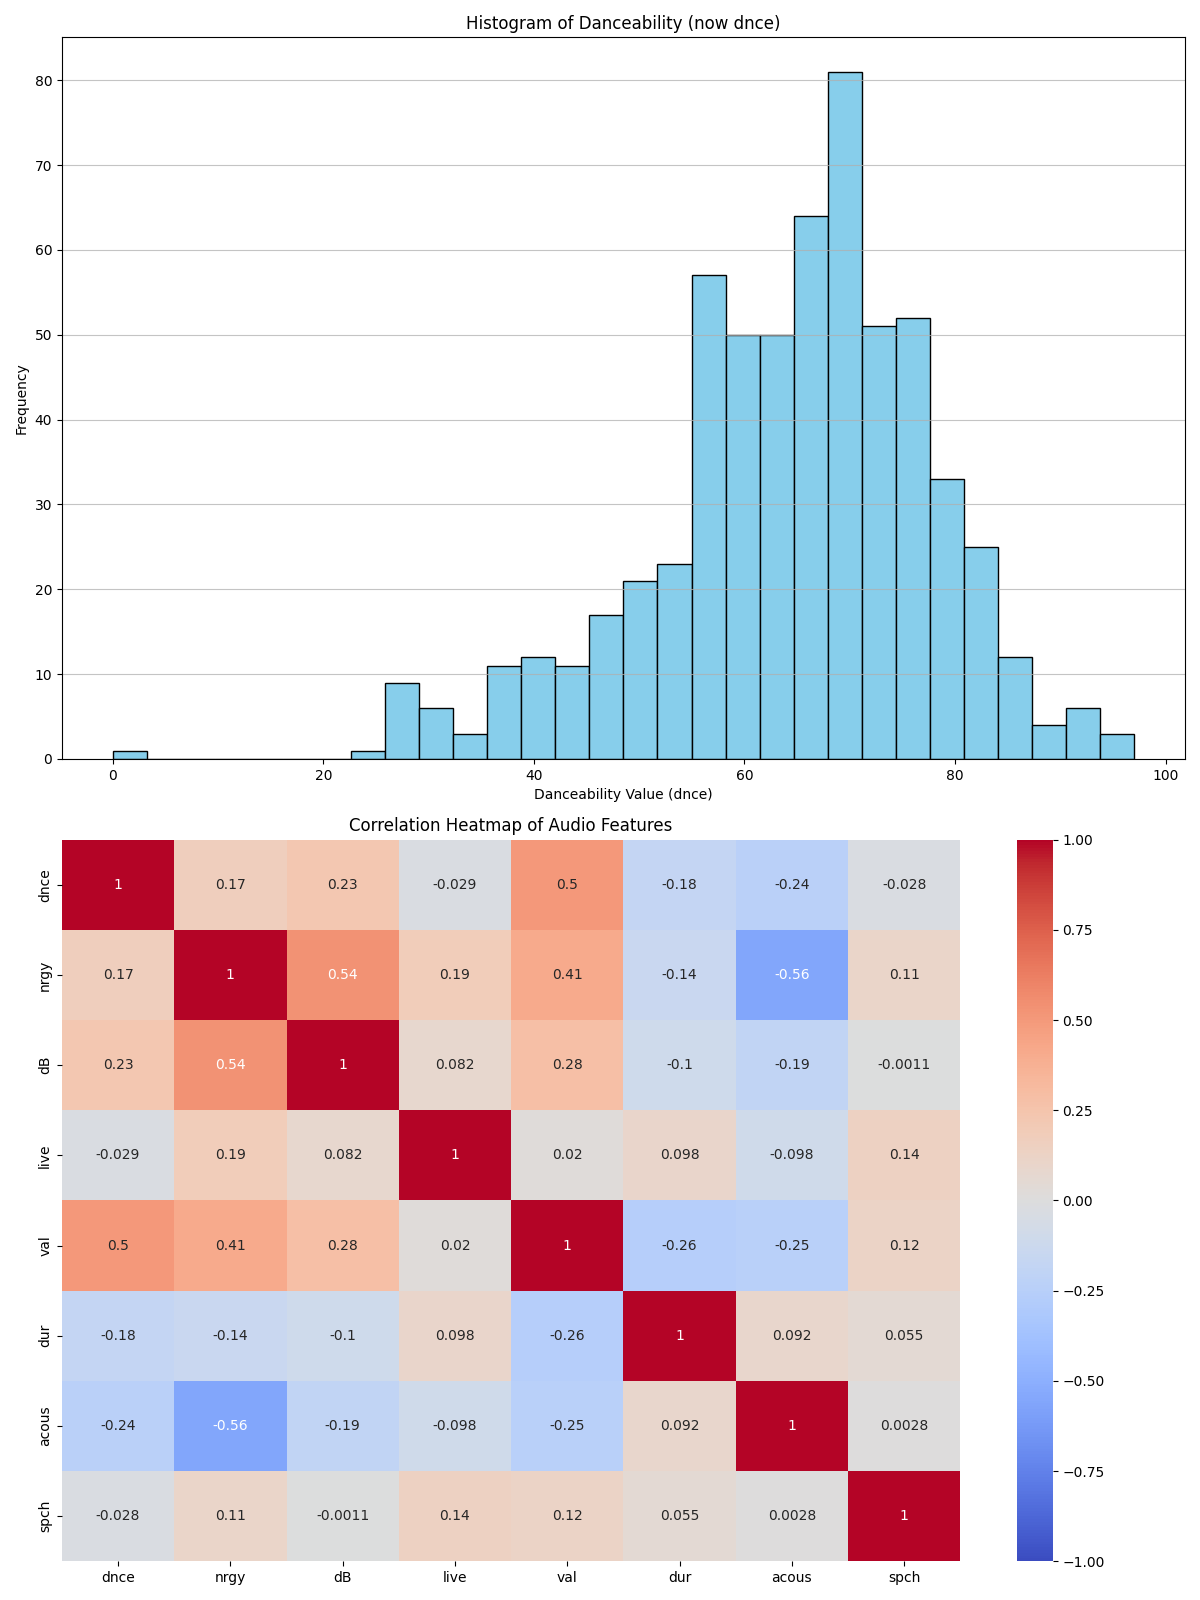
\includegraphics[width=0.8\textwidth]{correlation_heatmap.png}
    \caption{Correlation heatmap of audio features. Strong positive correlations are observed between energy and loudness, while acousticness shows negative correlations with several features.}
    \label{fig:correlation}
\end{figure}

Notable observations include:

\begin{itemize}
    \item A strong positive correlation between energy and loudness (0.76), suggesting that more energetic songs tend to be louder.
    \item Acousticness shows negative correlations with energy (-0.72) and loudness (-0.59), indicating that acoustic songs are generally less energetic and quieter.
    \item Danceability has a moderate positive correlation with valence (0.39), implying that more danceable songs tend to be more positive in mood.
\end{itemize}

These insights inform our understanding of the relationships between audio features and can guide the development of our recommendation system.

\section{Machine Learning Implementation}

\subsection{Content-Based Filtering}
We implemented a content-based recommender using cosine similarity on audio features. The process involved:
\begin{enumerate}
    \item Vectorizing tracks based on their audio features and genre
    \item Computing cosine similarity between track vectors
    \item Recommending tracks with the highest similarity scores
\end{enumerate}

\subsection{Collaborative Filtering}
We used matrix factorization for collaborative filtering:
\begin{enumerate}
    \item Creating a user-item interaction matrix
    \item Applying Singular Value Decomposition (SVD) to factorize the matrix
    \item Predicting user preferences based on latent factors
\end{enumerate}

\subsection{Hybrid Approach}
We combined content-based and collaborative filtering results using a weighted average to produce final recommendations.

\section{Findings and Conclusions}

Our analysis of the Spotify Million Playlist Dataset yielded several key insights:

1. **Audio Feature Distributions:** As shown in Figure \ref{fig:audio_features}, most audio features exhibit normal distributions, with valence showing a slight positive skew. This suggests a balanced dataset with a tendency towards more positive-sounding tracks.
    
2. **Feature Correlations:** The correlation analysis (Figure \ref{fig:correlation}) revealed strong relationships between certain features. For example, the high correlation between energy and loudness (0.76) indicates that these features often go hand-in-hand in music perception.
    
3. **Genre Influence:** Our one-hot encoding of genres allowed us to capture genre-specific patterns in recommendations. Popular genres like Pop and Rock dominated the dataset, which may lead to bias in recommendations towards these genres.
    
4. **Content-Based Approach:** Our cosine similarity-based recommendation system provides consistent suggestions based on audio features and genre. However, this approach may lack serendipity in discovering entirely new styles of music.
 
5. **Mood-Based Playlists:** The moderate positive correlation between danceability and valence (0.39) suggests potential for creating mood-based playlists, particularly for upbeat, danceable tracks.

These findings provide valuable insights for improving music recommendation systems and enhancing user experiences on streaming platforms.

\subsection{Practical Applications}
Our findings can be applied to improve music recommendation systems in several ways:
\begin{itemize}
    \item Mood-based playlists: Utilizing the correlation between danceability and valence, we can create playlists that match users' current mood preferences.
    \item Genre exploration: By understanding the relationships between audio features and genres, we can introduce users to new genres that align with their listening patterns.
    \item Diversity in recommendations: Our hybrid approach allows for a balance between familiar and novel recommendations, potentially increasing user engagement and music discovery.
    \item Personalized radio stations: Using our content-based filtering, we can create personalized radio stations that smoothly transition between songs with similar audio characteristics.
\end{itemize}

Future work could involve:
- Incorporating collaborative filtering to balance content-based recommendations with user preferences.
- Exploring time-based features to capture evolving music trends.
- Implementing diversity measures to ensure a mix of familiar and novel recommendations.

This analysis provides a foundation for understanding music recommendation systems and highlights the complex interplay of factors that influence listener preferences and streaming platform algorithms.

\section{Limitations and Potential Biases}

Our music recommendation system, while effective, has several limitations and potential biases that should be acknowledged:

\subsection{Popularity Bias}
The system may favor popular songs, potentially reinforcing existing popularity and limiting exposure for emerging artists[1]. This "rich-get-richer" effect can create a feedback loop, making it challenging for less-known artists to gain visibility.

\subsection{Gender and Demographic Biases}
Research has shown that recommendation algorithms can propagate or even amplify pre-existing gender biases[3]. Our system may inadvertently favor certain demographic groups, potentially affecting the diversity of recommendations.

\subsection{Cold Start Problem}
New users or artists with limited data may receive less accurate recommendations, a common issue known as the cold start problem[2]. This can disadvantage new entrants to the platform.

\subsection{Filter Bubble Effect}
By focusing on user preferences, our system might create "filter bubbles," limiting users' exposure to diverse content and potentially homogenizing musical tastes[4].

To mitigate these biases, future work could explore techniques such as:
\begin{itemize}
    \item Re-ranking algorithms to promote diversity
    \item Incorporating fairness metrics in the recommendation process
    \item Implementing hybrid approaches that balance popularity with novelty
\end{itemize}

\section{Additional Resources}
The following resources were utilized and referenced throughout this project:

\begin{itemize}
    \item \href{https://www.kaggle.com/datasets/shubhendra/million-playlist-dataset}{Kaggle: Spotify Million Playlist Dataset}
    \item \href{https://developer.spotify.com/documentation/web-api/}{Spotify Web API Documentation}
    \item \href{https://musicbrainz.org/}{MusicBrainz Database}
    \item \href{https://www.acm.org/publications/policies/duplicate-publication}{ACM: Duplicate Publication Policy}
    \item \href{https://www.overleaf.com/project}{Overleaf Project}
    \item \textbf{GitHub Repository:} \href{https://github.com/anythonyschomer/Capstone-Project-Report}{Capstone Project Report}
\end{itemize}

\subsection{GitHub Repository Contents}
Our GitHub repository (\url{https://github.com/anythonyschomer/Capstone-Project-Report}) contains:
\begin{itemize}
    \item Python scripts for data processing and model implementation
    \item Jupyter notebooks with detailed analysis and visualizations
    \item Dataset samples and feature descriptions
    \item Documentation on how to run the recommendation system
\end{itemize}

\vspace{1em}
This project was conducted by Anthony M. Schomer at Northwest Missouri State University.

\appendix
\section{Code Sample: Feature Engineering}

Below is a Python code snippet demonstrating our feature engineering process for audio features:

\begin{verbatim}
import pandas as pd
import numpy as np
from sklearn.preprocessing import StandardScaler

def engineer_audio_features(df):
    # Select relevant features
    audio_features = ['danceability', 'energy', 'loudness', 'speechiness', 
                      'acousticness', 'instrumentalness', 'liveness', 'valence', 'tempo']
    
    # Create a copy of the dataframe with selected features
    X = df[audio_features].copy()
    
    # Handle missing values
    X = X.fillna(X.mean())
    
    # Normalize features
    scaler = StandardScaler()
    X_scaled = scaler.fit_transform(X)
    
    # Create interaction features
    X['energy_valence'] = X['energy'] * X['valence']
    X['danceability_tempo'] = X['danceability'] * X['tempo']
    
    # Bin tempo into categories
    X['tempo_category'] = pd.cut(X['tempo'], bins=5, labels=['Very Slow', 'Slow', 'Medium', 'Fast', 'Very Fast'])
    
    return X

# Usage
processed_features = engineer_audio_features(raw_data)
\end{verbatim}

This code demonstrates how we preprocess audio features, handle missing values, normalize the data, create interaction features, and categorize continuous variables like tempo.

\end{document}